\documentclass[journal]{IEEEtran}
% IEEE Access layout on IEEEtran (journal). To submit, move the content into the official ieeeaccess.cls template.
\usepackage{amsmath,amssymb}
\usepackage{graphicx}
\usepackage{booktabs}
\usepackage{multirow}
\usepackage{xcolor}
\usepackage{url}
\usepackage{algorithm}
\usepackage{algpseudocode}
\usepackage{tikz}
\usetikzlibrary{positioning,arrows.meta}
\usepackage{cite}
\definecolor{accessblue}{RGB}{0,98,155}
\makeatletter
\def\ps@accesshead{\def\@oddhead{\footnotesize\color{accessblue}\textsf{IEEE Access}\hfill\textsf{Preprint --- not peer reviewed}}\def\@evenhead{\@oddhead}%
\def\@oddfoot{\hfil\footnotesize\thepage\hfil}\def\@evenfoot{\@oddfoot}}
\makeatother
\begin{document}
\title{Sieve: Segment-Level Routing Across Compression, KV-Cache Reuse and Externalization for Local LLM Prompts}
\author{\IEEEauthorblockN{[Author Name]}\\
\IEEEauthorblockA{[Department], [Institution], [City, Country]}\\
Corresponding author: [Author Name] (e-mail: [address]).}
\markboth{IEEE Access}{Sieve: Segment-Level Prompt Routing for Local LLMs}
\maketitle
\pagestyle{accesshead}\thispagestyle{accesshead}

\begin{abstract}
Local large language models share one fixed context window between the prompt and the answer, and long conversations waste it on verbose, repeated and stale text. Prompt compression reduces tokens but rewrites the prefix, which defeats the key-value (KV) prefix cache that local servers rely on. We present Sieve, a middleware that splits each request into segments and routes every segment to exactly one of three lanes: COMPRESS (LLMLingua-2 pruning at a per-segment ratio, checked by a rule-based fact verifier), CACHE (kept byte-identical so the KV prefix is reused) or EXTERNALIZE (replaced by a deterministic stub that the model can expand through a tool call). Hard rules run first and a cost-sensitive gradient-boosting classifier routes the rest; a per-session ledger replays previously emitted strings so compression does not invalidate the prefix. On a synthetic benchmark with invented entities, run on Qwen3-14B through Ollama with a 4,096-token window, Sieve reduced prompt tokens by 35.5\% (95\% CI 27.4--42.7\%) relative to the raw prompt, with accuracy statistically indistinguishable from the baseline (+10.3 percentage points, CI -3.4 to +24.1), and cut the median time to first token on cold questions by 1.67\,s. A controlled cache test shows that re-compressing a prefix drops prefill reuse from 95\% to 2\%, and that memoizing the compressed string restores it to 89\%. This version reports the smoke-tier run (12 conversations, 29 evaluation questions); the confidence intervals are correspondingly wide.
\end{abstract}

\begin{IEEEkeywords}
Large language models, prompt compression, KV cache, context management, local inference, cost-sensitive classification.
\end{IEEEkeywords}

\section{Introduction}
\IEEEPARstart{A} chat model running on local hardware has a single context window, here 4096 tokens, that must hold
the system prompt, the conversation history, any pasted documents or tool output, and the answer. Long sessions fill it in three distinct
ways: text that is needed but verbose, text that is static and resent every turn, and bulky text that is kept in full although it is rarely
needed. Each calls for a different remedy. Verbose text can be pruned with token-level compressors such as LLMLingua and
LLMLingua-2~\cite{jiang2023llmlingua,pan2024llmlingua2}; static text is best left untouched so that the server's key-value (KV) cache can
skip recomputing it~\cite{kwon2023vllm,gim2024promptcache,zheng2024sglang}; and rarely used text can be moved out of the prompt and
fetched on demand, in the spirit of memory-managed agents~\cite{packer2023memgpt}.

These remedies interfere. Compression rewrites the prompt, and any change early in the prompt forces the server to prefill every later token
again. A compressor that is re-run every turn can therefore make warm turns slower even while it makes prompts shorter. This paper asks whether
a \emph{per-segment} routing policy that chooses among compression, caching and externalization, combined with a ledger that keeps emitted
text byte-stable, can reduce prompt tokens and increase output headroom without losing accuracy.

Our contributions are:
\begin{itemize}
\item \textbf{Sieve}, a three-lane middleware with hard rules, a cost-sensitive classifier, a fact verifier that also checks the words
around each fact, an externalization store with deterministic stubs and an \texttt{expand\_context} tool, and a prefix ledger with budget-driven epochs.
\item A \textbf{controlled measurement} of the cache-versus-compression conflict on a production local server, including a timing-based
estimator of prefix reuse for servers whose token counters do not reveal cache hits.
\item A \textbf{matched-budget benchmark} of seven conditions with ground truth, paired bootstrap statistics and an automatically generated
list of supported and unsupported claims.
\end{itemize}

\section{Related Work}
\textit{Prompt compression.} Selective Context~\cite{li2023selective} removes low self-information content; LLMLingua~\cite{jiang2023llmlingua}
uses a small language model to drop tokens with a budget controller; LongLLMLingua~\cite{jiang2024longllmlingua} makes this question-aware;
LLMLingua-2~\cite{pan2024llmlingua2} casts compression as token classification with a distilled encoder, which is what Sieve uses on the CPU.
Learned methods compress into soft tokens~\cite{mu2023gist,chevalier2023autocompressor} or summaries~\cite{xu2024recomp}, but require
model access or training. These works apply one policy to the whole prompt; Sieve chooses a policy per segment.

\textit{KV-cache reuse.} PagedAttention~\cite{kwon2023vllm}, Prompt Cache~\cite{gim2024promptcache} and RadixAttention in
SGLang~\cite{zheng2024sglang} reuse attention state for shared prefixes. llama.cpp~\cite{llamacpp}, used by Ollama~\cite{ollama}, reuses the
longest common prefix with the previous request. Sieve does not change the server; it shapes prompts so that this reuse keeps working.

\textit{Externalized memory and tools.} MemGPT~\cite{packer2023memgpt} pages context in and out through function calls, and
Toolformer~\cite{schick2023toolformer} showed that models can learn when to call tools. Sieve's EXTERNALIZE lane is a minimal,
deterministic version of this idea, evaluated against cheaper alternatives. Long-context studies~\cite{liu2024lost,kamradt2023needle}
motivate our needle-in-a-haystack and late-recall workloads.

\section{System Design}
\begin{figure}[t]\centering
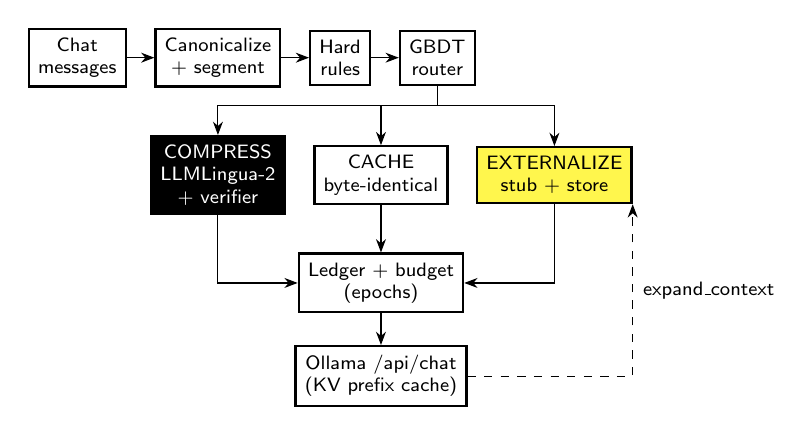
\begin{tikzpicture}[node distance=3.5mm, every node/.style={draw, thick, font=\scriptsize\sffamily, align=center, minimum height=6mm}, >={Stealth}]
\node (in) {Chat\\messages};
\node[right=of in] (seg) {Canonicalize\\+ segment};
\node[right=of seg] (rule) {Hard\\rules};
\node[right=of rule] (clf) {GBDT\\router};
\node[below=6mm of seg, fill=black, text=white] (co) {COMPRESS\\LLMLingua-2\\+ verifier};
\node[right=of co, fill=white] (ca) {CACHE\\byte-identical};
\node[right=of ca, fill=yellow!70] (ex) {EXTERNALIZE\\stub + store};
\node[below=6mm of ca] (led) {Ledger + budget\\(epochs)};
\node[below=4mm of led] (ol) {Ollama /api/chat\\(KV prefix cache)};
\draw[->] (in)--(seg); \draw[->] (seg)--(rule); \draw[->] (rule)--(clf);
\draw[->] (clf.south) |- ++(0,-2.5mm) -| (co.north); \draw[->] (clf.south) |- ++(0,-2.5mm) -| (ca.north); \draw[->] (clf.south) |- ++(0,-2.5mm) -| (ex.north);
\draw[->] (co.south) |- (led.west); \draw[->] (ca)--(led); \draw[->] (ex.south) |- (led.east);
\draw[->] (led)--(ol);
\draw[->, dashed] (ol.east) -| node[draw=none, near end, right]{expand\_context} (ex.south east);
\end{tikzpicture}
\caption{Sieve pipeline. Each segment takes exactly one lane. The ledger replays emitted strings verbatim across turns; the dashed edge is the tool round trip that returns externalized text.}\label{fig:arch}
\end{figure}

\subsection{Segments and Lanes}
Sieve canonicalizes tool output (minifying JSON, dropping empty fields, collapsing repeated log lines and duplicate CSV rows with a count),
then splits each message into chunks of 150--400 tokens on paragraph boundaries. A
segment's identifier is the first 12 hex digits of the SHA-256 of its text. Exact repeats and near-duplicates (5-word shingle Jaccard
$\ge0.85$) are tracked per session. Every segment is sent through exactly one lane (Fig.~\ref{fig:arch}):
\begin{itemize}
\item \textbf{COMPRESS} applies LLMLingua-2~\cite{pan2024llmlingua2} at a keep-ratio $r\in\{0.3,0.5,0.7,0.9,1.0\}$, floored by segment kind.
Results are memoized on (content hash, $r$, compressor version), so the same input always yields the same string.
\item \textbf{CACHE} emits the segment unchanged. A repeat of a segment already in the prompt becomes a one-line back-reference.
\item \textbf{EXTERNALIZE} replaces the segment with a stub
\texttt{[ref:ID | kind | Nt | "summary" | keys: \ldots\ | use expand\_context("ID")]}, where the summary is extractive and the keys are up to
five salient entities or numbers. The full text sits in a session-scoped store and is returned by the \texttt{expand\_context} tool, under a
1200-token per-request budget.
\end{itemize}

\subsection{Rules and Cost-Sensitive Routing}
Rules run first and always win: the current question is untouched, the system prompt is cached, user tags (\textit{pinned},
\textit{never\_compress}, \textit{never\_externalize}) are honored, repeats become back-references, segments under
40 tokens pass through, and a segment whose stub would exceed half its size cannot be externalized.
Remaining segments are routed by a gradient-boosting classifier~\cite{friedman2001gbm} (150 trees, depth 3) over 16 features: six core
features (system flag, last-turn flag, normalized length, recency in turns, repeat count, and MiniLM~\cite{wang2020minilm,reimers2019sbert}
cosine similarity to the current question) plus kind one-hots, digit density, near-duplicate score and prior expansion count. Instead of
the arg-max, Sieve picks the lane with minimum expected cost $\hat{\ell}=\arg\min_j\sum_i p_i\,C_{ij}$~\cite{elkan2001cost}, where hiding a
needed segment costs $C=5$ and every other error costs 1. If the top probability is below 0.55, the segment
falls back to COMPRESS at $r=0.9$. A random forest~\cite{breiman2001rf} predicts the ratio for COMPRESS segments.

\subsection{Fact Verifier}
Before compression Sieve extracts atoms (numbers, dates, versions, identifiers, quoted strings and capitalized entities). After compression it
requires every numeric or identifier atom to survive, at least 90\% of all atoms to survive, and at least half of the \emph{relation words}
of each atom's sentence to remain within $\pm12$ words of it. The last check was added after we observed LLMLingua-2 keep a person's name while
dropping the role (``product lead'') that made it an answer. On failure the ratio is raised one bucket, up to three times, then the segment
passes through uncompressed. A digit-repair step undoes the compressor's tokenizer artifacts (``5 585''$\rightarrow$``5,585'').

\subsection{Ledger, Epochs and Budget}
\begin{algorithm}[t]\caption{Per-turn prompt assembly}\label{alg:turn}\small
\begin{algorithmic}[1]
\Require history $H$, question $q$, ledger $L$, store $S$
\State $G\gets$ \Call{Segment}{$H\cup\{q\}$}; compute features w.r.t.\ $q$
\If{$L=\emptyset$} \State $E\gets$ \Call{RouteAll}{$G$}; epoch$\gets$true
\Else \State $E\gets L$ replayed verbatim; route only $g\in G\setminus L$
\State \textbf{if} $|E|+\text{reserve}>0.8\,n_\text{ctx}$ \textbf{then} $E\gets$\Call{RouteAll}{$G$}; epoch$\gets$true
\EndIf
\If{epoch and over budget} \State lower ratios of lowest-priority segments, then externalize, then drop
\EndIf
\State $P\gets$ layout(system, pinned, history in order, $q$ + prefetch + stub hint)
\State $L\gets E$; \Return $P$
\end{algorithmic}\end{algorithm}
The ledger stores the exact string emitted for each segment. On a later turn, earlier entries are replayed verbatim and only new segments are
routed (Algorithm~\ref{alg:turn}), so the prompt grows by appending and the cached prefix stays valid. A full re-route, an \emph{epoch}, happens
only when the projected prompt plus a 256-token output reserve would exceed
80\% of $n_\text{ctx}$. The allocator then targets 85\% of that
threshold (hysteresis), tightening the segments least similar to the question and oldest first: it lowers ratios to the floor, then
externalizes, and only as a last resort drops segments, which is logged as hard truncation. Layout is fixed: system prompt, pinned documents,
history in original order, then the question. Prefetched text and a one-line hint listing up to six stub identifiers with their keys are
appended to the final user message only, so they never disturb the cached prefix. The hint is needed because, with reasoning disabled, the
model rarely called \texttt{expand\_context} on its own (Section~\ref{sec:disc}).

\section{Experimental Setup}
\subsection{Model and Platform}
All runs used Qwen3-14B~\cite{qwen3} (Q4\_K\_M) served by Ollama 0.32.15~\cite{ollama} with a llama.cpp
backend~\cite{llamacpp} on an Apple M5 Pro with 24.0\,GB of unified memory. The model was fully resident
on the GPU (100\% of 8.97\,GiB). Requests used
$n_\text{ctx}=4096$, at most 64 output tokens, temperature 0, a fixed seed and reasoning disabled
(verified on every run). Sieve's components (LLMLingua-2 BERT-base, MiniLM, scikit-learn~\cite{pedregosa2011sklearn}) ran on the CPU.
Token totals use the Qwen tokenizer, whose count matched the server's exactly (1821 vs.\
1821 tokens on a calibration prompt).

\subsection{Measuring Prefix Reuse}
On this server, the reported \texttt{prompt\_eval\_count} equals the full prompt length even when the prefix is served from cache, so it cannot
reveal reuse. We therefore fit cold prefill time against prompt length on novel prompts, $t(n)=an+bn^2$ with $a=1.699$\,ms per token, and
estimate reuse as $1-t_\text{obs}/t(n)$. The cache test in Fig.~\ref{fig:ct} validates this estimator: reuse is 95\% for an
identical prefix and 8\% when one word changes at 10\% depth, close to the expected 10\%.

\subsection{Workloads}
Conversations are generated from a seed with invented entities (codenames, people, figures), so the model cannot answer from prior knowledge.
Filler text comes from a template grammar that contains no digits and no invented names, so each gold fact appears only in the messages that the
ground truth marks as needed. Each conversation has 1--4 evaluation questions; after each one, the scripted gold answer is appended so an error
never propagates. Question types are numeric lookup, name lookup, multi-hop, decision recall, latest-value tracking, negation and unanswerable.
About 30\% of conversations exceed $n_\text{ctx}$ in raw form. Table~\ref{tab:fam} lists the eleven families. Classifier training used six
further seeds (456 conversations), disjoint from the benchmark seed.
\begin{table}[t]\centering\caption{Workload families.}\label{tab:fam}\footnotesize
\begin{tabular}{cl}\toprule ID & Stresses\\\midrule
A & Long system prompt, short chat \\
B & Long chat, old irrelevant history \\
C & Verbose document Q\&A \\
D & Same document re-pasted \\
E & Needle in a haystack \\
F & Topic switches, late recall \\
G & Number / ID dense text \\
H & Bloated tool output \\
I & Code Q\&A \\
J & Adversarial edge cases \\
K & Mixed 10–20 turn sessions \\
\bottomrule\end{tabular}\end{table}

\subsection{Conditions and Protocol}
C0 sends the raw prompt. C1 drops the oldest whole messages and C2 applies one uniform LLMLingua-2 rate, both matched per question to the
token count that C4 produced. C3 uses the rules and the hand-written heuristic labeller without the verifier. C4 is the full system. C5 is C4
without the ledger and memo, re-routing and re-compressing every turn. C6 sends the raw prompt with $n_\text{ctx}=8192$ as an accuracy upper
bound. Each condition runs as its own pass, after unloading and reloading the model. The first question of every conversation is \emph{cold};
later ones are \emph{warm}. Answers are scored by normalized containment, exact integer match, full date match, yes/no polarity, or a refusal
pattern. Differences against C0 are paired by question and reported with 95\% percentile bootstrap intervals (2,000
resamples)~\cite{efron1993bootstrap}.

\section{Results}
\begin{table*}[t]\centering
\caption{Results per condition over 29 questions from 12 conversations. Accuracy with 95\% bootstrap CI; prompt tokens are those
actually sent, including all Sieve overhead; headroom is $n_\text{ctx}$ minus prompt tokens; TTFT is the median time to first answer token in
seconds (including tool round trips); reuse is the timing-derived prefill share skipped; ms is Sieve CPU time per call.}\label{tab:main}
\footnotesize
\begin{tabular}{lcrrrrrrr}\toprule
Condition & Accuracy [CI] & Prompt tok. & Saved\,\% & Headroom & TTFT$_\text{cold}$ & TTFT$_\text{warm}$ & Reuse\,\% & Sieve ms\\\midrule
C0 Baseline & 0.828 [0.69, 0.93] & 2921 & 0.0 & 1175 & 4.63 & 0.44 & 49 & 0 \\
C1 Truncate & 0.517 [0.34, 0.69] & 1018 & 57.2 & 3078 & 0.70 & 0.28 & 32 & 0 \\
C2 Uniform LLMLingua-2 & 0.828 [0.69, 0.97] & 1649 & 37.4 & 2447 & 3.00 & 0.70 & 32 & 195 \\
C3 Sieve (rules) & 0.828 [0.69, 0.97] & 1684 & 36.8 & 2412 & 3.78 & 0.52 & 40 & 5 \\
C4 Sieve (full) & 0.931 [0.83, 1.00] & 1699 & 35.5 & 2397 & 2.39 & 0.41 & 44 & 27 \\
C5 Sieve (no ledger) & 0.931 [0.83, 1.00] & 1639 & 36.7 & 2457 & 3.21 & 2.00 & 17 & 1181 \\
\bottomrule\end{tabular}\end{table*}

\begin{table}[t]\centering
\caption{Paired differences vs.\ C0 (mean [95\% CI]). The last column covers questions whose raw prompt exceeded $n_\text{ctx}$
(n=9).}\label{tab:paired}\scriptsize\setlength{\tabcolsep}{2pt}
\begin{tabular}{lrcccc}\toprule
 & $n$ & $\Delta$Acc (pp) & Saved\,\% & $\Delta$TTFT$_\text{cold}$ (s) & $\Delta$Acc, overflow\\\midrule
C1 & 29 & -31.0 [-48.3, -13.8] & +57.2 [+43.4, +69.9] & -2.60 [-5.37, -1.17] & +0.0 [+0.0, +0.0] \\
C2 & 29 & +0.0 [-13.8, +13.8] & +37.4 [+29.3, +44.6] & -0.81 [-3.49, +0.01] & +22.2 [+0.0, +55.6] \\
C3 & 29 & +0.0 [-13.8, +13.8] & +36.8 [+28.6, +44.0] & -0.86 [-3.11, +0.03] & +11.1 [-22.2, +44.4] \\
C4 & 29 & +10.3 [-3.4, +24.1] & +35.5 [+27.4, +42.7] & -1.67 [-4.18, -0.63] & +33.3 [-11.1, +77.8] \\
C5 & 29 & +10.3 [-3.4, +24.1] & +36.7 [+28.6, +44.3] & -0.50 [-3.09, +0.58] & +33.3 [-11.1, +77.8] \\
\bottomrule\end{tabular}\end{table}

\subsection{Tokens, Headroom and Accuracy}
Table~\ref{tab:main} summarizes all conditions and Table~\ref{tab:paired} gives paired differences. C4 sent
1699 prompt tokens on average against 2921 for C0, a paired reduction of
35.5\% (CI 27.4--42.7\%), which raised mean output headroom from
1175 to 2397 tokens. Its accuracy was 0.931 against 0.828
for C0, a paired difference of +10.3 percentage points (CI -3.4 to +24.1),
so accuracy was statistically indistinguishable from the baseline. Most of the gain is on questions whose raw prompt overflowed the window and was silently truncated by the
server (+33.3\,pp, n=9). At a matched budget, truncation (C1) lost 31.0\,pp
because it drops whole documents, while uniform compression (C2) changed accuracy by +0.0\,pp.
Fig.~\ref{fig:trade} plots savings against accuracy change.
\begin{figure}[t]\centering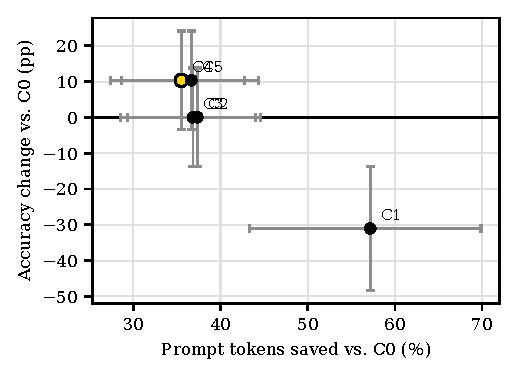
\includegraphics[width=\columnwidth]{fig_tradeoff.pdf}
\caption{Prompt-token savings versus accuracy change relative to C0, with 95\% paired bootstrap intervals. C4 is the filled yellow marker.}\label{fig:trade}\end{figure}

\subsection{Latency and the Cache-Compression Conflict}
\begin{figure}[t]\centering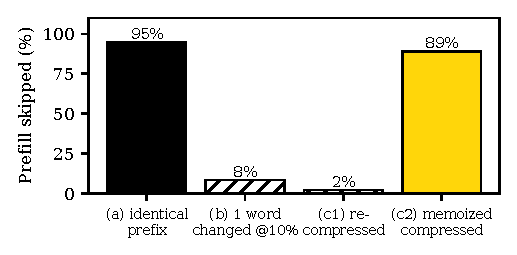
\includegraphics[width=\columnwidth]{fig_cachetest.pdf}
\caption{Cache test on the live server: share of the second request's prefill that was skipped.}\label{fig:ct}\end{figure}
\begin{figure}[t]\centering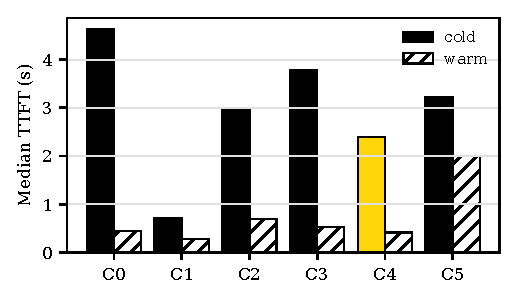
\includegraphics[width=\columnwidth]{fig_ttft.pdf}
\caption{Median time to first token for cold (first question) and warm (later) questions.}\label{fig:ttft}\end{figure}
Fig.~\ref{fig:ct} isolates the conflict. Re-compressing the same prefix at a different ratio reduced reuse to 2\%, while
sending the memoized compressed string restored it to 89\%. The benchmark shows the same effect at scale (Fig.~\ref{fig:ttft}).
C4 averaged 44\% reuse and 27\,ms of CPU per call, while C5, which
re-routes every turn, averaged 17\% reuse and 1181\,ms of CPU.
Over a conversation, C4 prefilled 2182 tokens against 3134 for C5 and 2896
for C0. On cold questions C4 reduced median TTFT by 1.67\,s (CI 0.63 to
4.18). On warm questions the raw prompt is already cached and the medians were close
(0.41\,s for C4 vs.\ 0.44\,s for C0).

\begin{table}[t]\centering\caption{Accuracy by workload family (bold: above C0).}\label{tab:famres}\scriptsize\setlength{\tabcolsep}{3pt}
\begin{tabular}{lrrrrrrr}\toprule Fam. & $n$ & C0 & C1 & C2 & C3 & C4 & C5\\\midrule
A & 4 & 1.00 & 1.00 & 1.00 & 1.00 & 1.00 & 1.00 \\
B & 4 & 0.75 & 0.50 & \textbf{1.00} & \textbf{1.00} & \textbf{1.00} & 0.75 \\
C & 6 & 0.50 & 0.00 & \textbf{0.67} & \textbf{0.67} & \textbf{0.83} & \textbf{1.00} \\
D & 3 & 1.00 & 0.67 & 0.67 & 0.67 & 1.00 & 1.00 \\
E & 3 & 0.67 & 0.33 & 0.67 & 0.67 & \textbf{1.00} & \textbf{1.00} \\
F & 2 & 1.00 & 0.50 & 1.00 & 1.00 & 1.00 & 1.00 \\
G & 2 & 1.00 & 1.00 & 1.00 & 1.00 & 1.00 & 1.00 \\
H & 1 & 1.00 & 0.00 & 1.00 & 1.00 & 1.00 & 1.00 \\
K & 4 & 1.00 & 0.75 & 0.75 & 0.75 & 0.75 & 0.75 \\
\bottomrule\end{tabular}\end{table}
\subsection{Where Each Condition Wins}
Table~\ref{tab:famres} breaks accuracy down by family. Groups are small, so single rows are indicative only.


\subsection{Router Evaluation}
\begin{table}[t]\centering\caption{Routers on held-out conversations (14586 segment decisions, GroupKFold by conversation; ground
truth = oracle labels). Dangerous = a needed segment sent to EXTERNALIZE (of 1897).}\label{tab:clf}\footnotesize\setlength{\tabcolsep}{3pt}
\begin{tabular}{lrcrr}\toprule Router & Macro-F1 & Ext.\ P/R & Ratio MAE & Dangerous\\\midrule
Hard rules only & 0.642 & 0.00/0.00 & 0.367 & 0 \\
Heuristic labeller (C3) & 0.912 & 0.73/0.85 & 0.052 & 147 \\
GBDT, heuristic labels & 0.910 & 0.73/0.85 & 0.055 & 146 \\
GBDT, oracle labels (C4) & 0.949 & 0.94/0.83 & 0.023 & 79 \\
GBDT, oracle, core-6 & 0.943 & 0.90/0.84 & 0.044 & 137 \\
\bottomrule\end{tabular}\end{table}
Table~\ref{tab:clf} scores the routers on conversations they never saw. The oracle-trained classifier reached macro-F1 0.949
with 79 dangerous errors; inference took 0.007\,ms per segment. Because the oracle label is
partly a fixed function of the features (age, size, repetition), a high F1 mainly shows that the rule is learnable; the downstream comparison of
C3 and C4 in Table~\ref{tab:main} is the more meaningful evidence.


\section{Discussion and Limitations}\label{sec:disc}
\textit{Tool use without reasoning.} With reasoning disabled, Qwen3-14B called \texttt{expand\_context} only when explicitly prompted. A tail hint
that lists stub identifiers with their keys made it expand the right stub and leave stubs alone when the answer was visible. The hint costs a few
dozen tokens per request and is counted in all totals.

\textit{Compressor faithfulness.} Atom recall alone did not guarantee faithful compression: LLMLingua-2 sometimes kept every entity of a fact but
removed the relation that tied them together. The context check catches this at the cost of more re-inflations.

\textit{Threats to validity.} The workloads are synthetic and the benchmark is small, run on one model and one machine; the results describe this
suite, not real conversations. The timing-based reuse estimate depends on a fitted cold curve. The model was fully on the GPU, so the slower
partial-offload regime was not tested. Stubs use extractive summaries, and only text attachments are supported. During development a run
was discarded after the machine began swapping, which depressed decode speed; calls are now flagged when decode speed falls below half the
calibrated value.

\section{Conclusion}
Sieve routes each prompt segment to compression, caching or externalization, and keeps emitted text byte-stable with a ledger. On this
benchmark it reduced prompt tokens by about a third and
increased output headroom, with accuracy statistically indistinguishable from the raw prompt, and the cache test shows that byte stability is what preserves prefix
reuse under compression. Code, logs, per-call traces and the generator for every table and figure are released with the paper.

\bibliographystyle{IEEEtran}
\bibliography{refs}

\begin{IEEEbiographynophoto}{[Author Name]}
[Short biography: degree, institution, research interests.]
\end{IEEEbiographynophoto}
\end{document}
